\documentclass{article}

\usepackage{graphicx}
\usepackage{tikz}
\usepackage{tikzsymbols}
\usetikzlibrary{calc,patterns,shapes.geometric}
\pagestyle{empty}
\usepackage[margin=0pt]{geometry}
\geometry{papersize={14in,12in}}

\def\centerarc[#1](#2)(#3:#4:#5){\draw[#1] ($(#2)+({#5*cos(#3)},{#5*sin(#3)})$) arc (#3:#4:#5);}

\begin{document}
	\begin{figure}
		\centering
		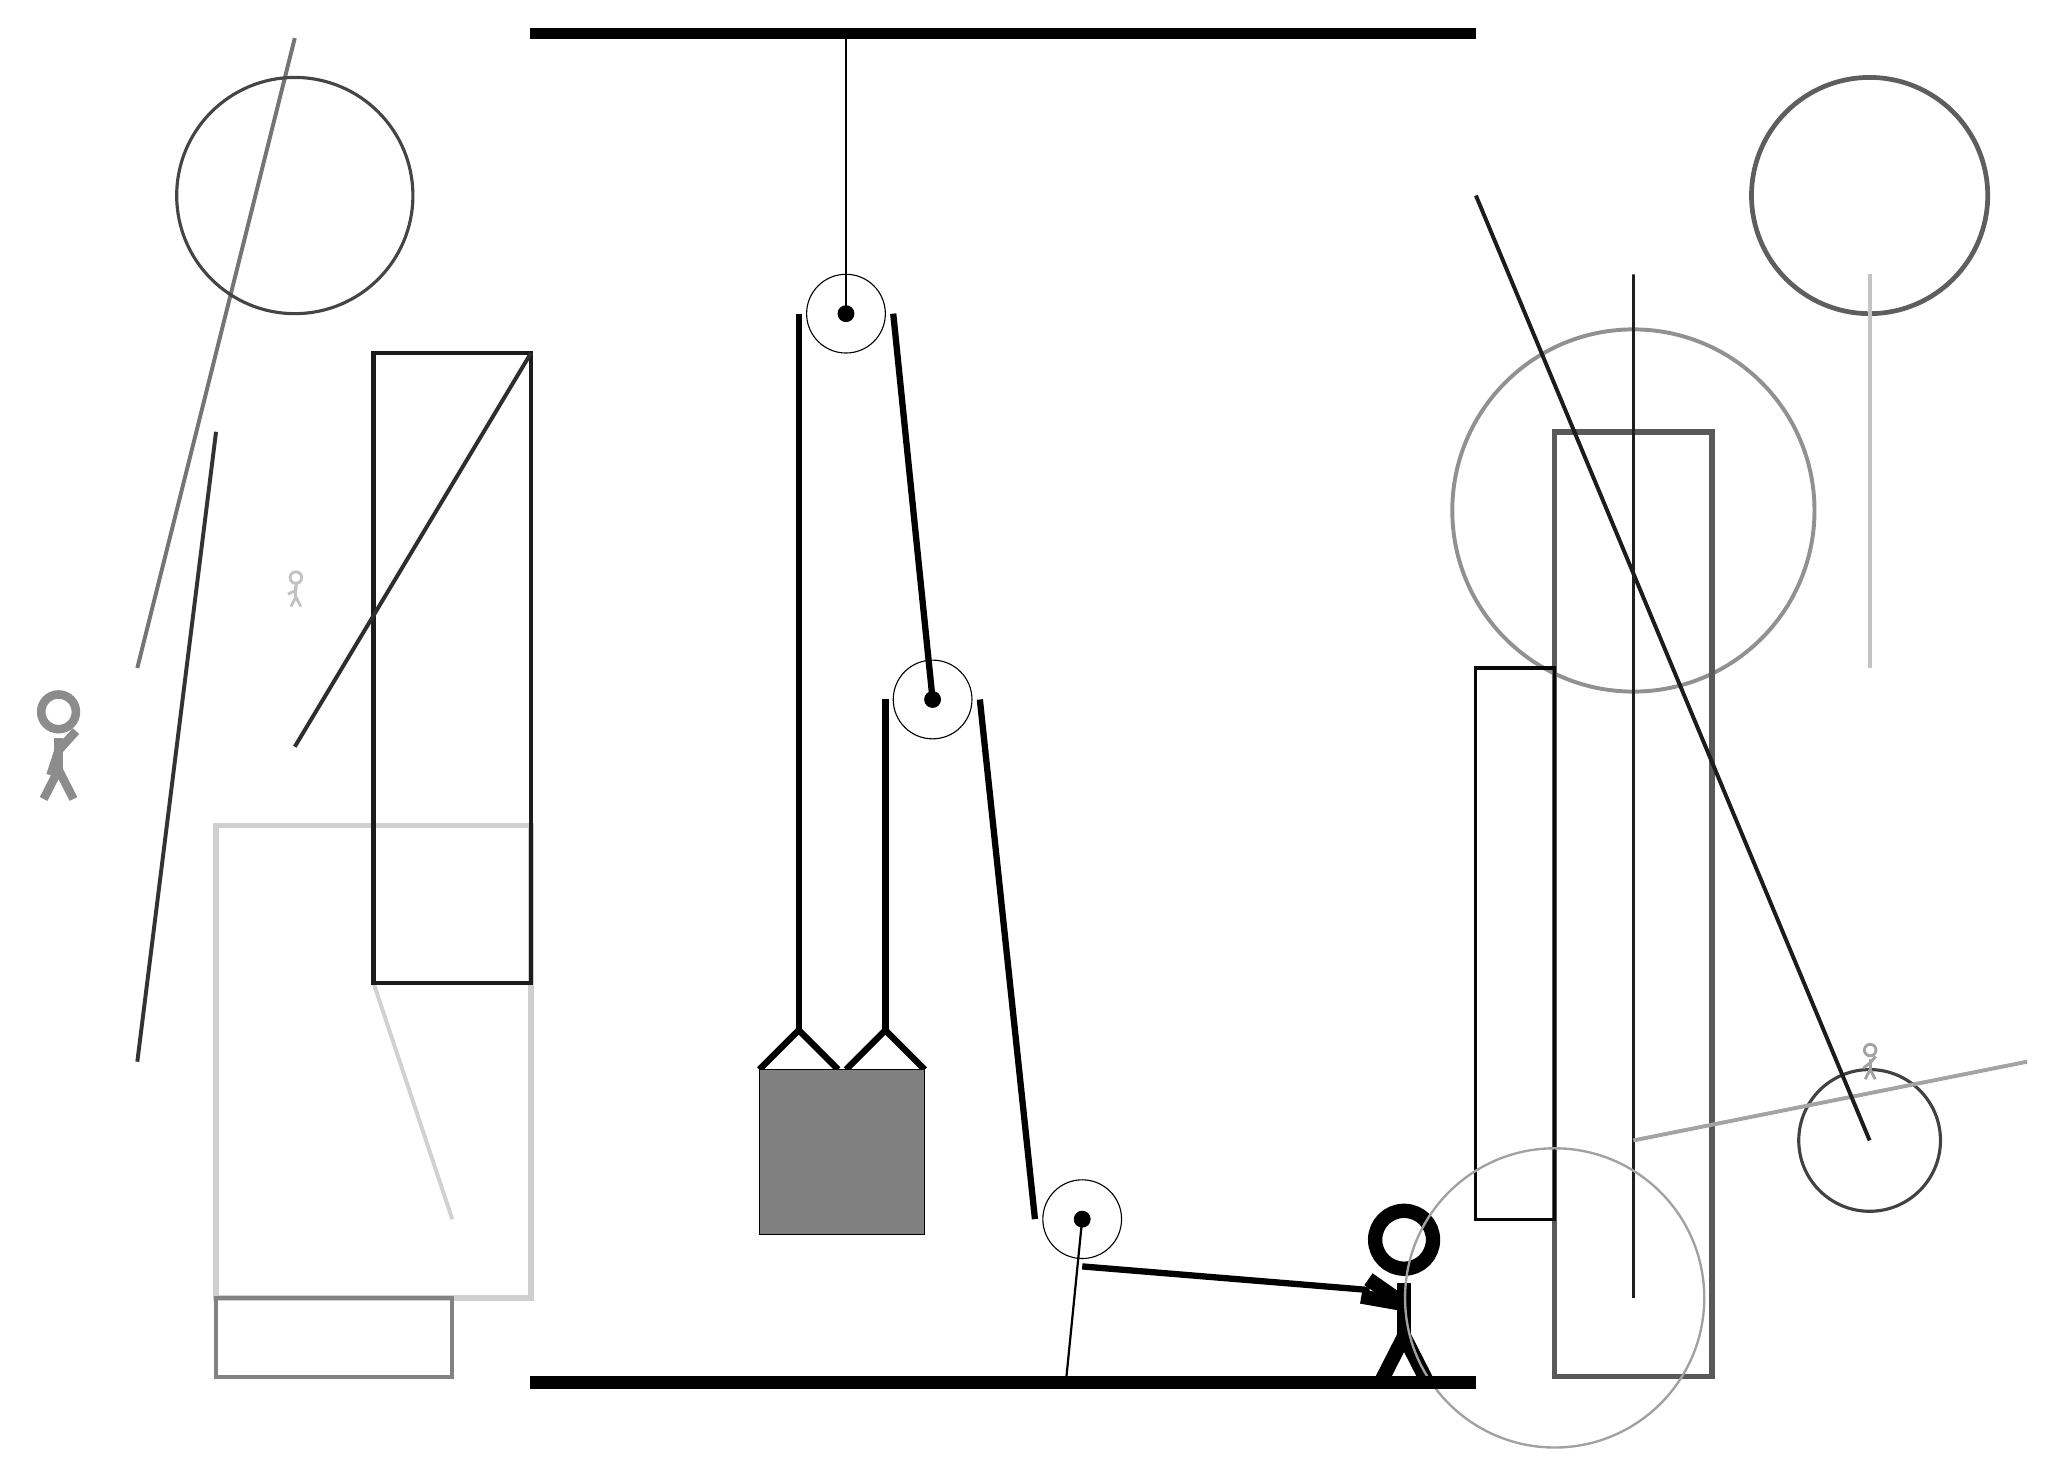
\begin{tikzpicture}
			%%%%% START %%%%%
			
			\draw[fill=black] (-2, 14) rectangle (10, 14.125);
			
			\draw (2, 10.5) circle (0.5);
			\draw[fill=black] (2, 10.5) circle (0.1);
			\draw[thick] (2, 10.5) -- (2, 14);
			
			\draw (3.1, 5.6) circle (0.5);
			\draw[fill=black] (3.1, 5.6) circle (0.1);
			
			\draw (5, -1) circle (0.5);
			\draw[fill=black] (5, -1) circle (0.1);
			\draw[thick] (5, -1) -- (4.8, -3);
			
			\draw[line width = 0.8mm]  (0.9, 0.9) -- (1.4, 1.4) -- (1.9, 0.9);
			\draw[line width = 0.8mm]  (2.0, 0.9) -- (2.5, 1.4) -- (3.0, 0.9);
			\draw[fill=black!50] (0.9, 0.9) rectangle (3.0, -1.2);
			
			\draw[line width = 0.8mm] (1.4, 10.5) -- (1.4, 1.4);
			\centerarc[line width = 0.8mm](2, 10.5)(0:180:0.6);
			\draw[line width = 0.8mm] (2.6, 10.5) -- (3.1, 5.6);
			\draw[line width = 0.8mm] (2.5, 5.6) -- (2.5, 1.4);
			\centerarc[line width = 0.8mm](3.1, 5.6)(0:180:0.6);
			\draw[line width = 0.8mm] (3.7, 5.6) -- (4.4, -1);
			\centerarc[line width = 0.8mm](5, -1)(180:270:0.6);
			\draw[line width = 0.8mm] (5, -1.6) -- (8.65, -1.9);
			
			\node at (9, -2) {\Strichmaxerl[10][-35][170]};
			
			\draw [line width=0.5mm, color=black!43](12, 8) circle (2.3);
			
			\draw[line width=0.7mm, color=black!65] (11, 9) rectangle (13, -3);
			\node[line width=0.3mm, color=black!24] at (-5, 7) {\Strichmaxerl[2][24][86]};
			\draw[line width=0.5mm, color=black!54](-5, 14) -- (-7, 6);
			
			\draw[line width=0.5mm, color=black!18](-4, 2) -- (-3, -1);
			\draw [line width=0.4mm, color=black!74](15, 0) circle (0.9);
			\draw[line width=0.4mm, color=black!88] (12, -2) rectangle (12, 11);
			
			\draw[line width=0.4mm, color=black!97] (10, 6) rectangle (11, -1);
			\draw [line width=0.6mm, color=black!63](15, 12) circle (1.5);
			
			\node[line width=0.7mm, color=black!45] at (-8, 5) {\Strichmaxerl[6][72][48]};
			\draw[line width=0.7mm, color=black!19] (-2, 4) rectangle (-6, -2);
			
			\draw[line width=0.5mm, color=black!80](-7, 1) -- (-6, 9);
			\draw[line width=0.5mm, color=black!36](12, 0) -- (17, 1);
			
			\draw [line width=0.3mm, color=black!37](11, -2) circle (1.9);
			\draw[line width=0.5mm, color=black!23](15, 6) -- (15, 11);
			\node[line width=0.4mm, color=black!36] at (15, 1) {\Strichmaxerl[2][37][50]};
			
			\draw[line width=0.6mm, color=black!89] (-2, 10) rectangle (-4, 2);
			
			\draw[line width=0.5mm, color=black!49] (-3, -2) rectangle (-6, -3);
			\draw[line width=0.5mm, color=black!82](-2, 10) -- (-5, 5);
			\draw[line width=0.5mm, color=black!89](10, 12) -- (15, 0);
			\draw [line width=0.4mm, color=black!73](-5, 12) circle (1.5);
			
			\draw[fill=black] (-2, -3) rectangle (10, -3.15);
			
			%%%%% END %%%%%
		\end{tikzpicture}
	\end{figure}	
\end{document}